\chapter{Linux Malware Analysis}
\thispagestyle{chapterfancy}

Malware analysis is the art of dissecting malware to understand how it works, how to identify it, and how to defeat or eliminate it. Malicious software, or malware, plays a part in most computer intrusion and security incidents. Any software that does something that causes harm to a user, computer, or network can be considered malware, including viruses, trojan horses and worms. While the various malware incarnations do all sorts of different things, there exist a core set of tools and techniques at our disposal for analyzing malware. \\
To be able to properly explain how Malware Analysis works, we will use the books "Practical Malware Analysis" by Michael Sikorski and Andrew Honig \cite{sikorski2012practical} and "Practical Binary Analysis" by Dennis Andriesse \cite{andriesse2018practical} \cite{prince2024understanding} as reference. \\

\section{Type of Malware}
There are various categories of malware, each with its own characteristics and methods of attack. Here are some common malware categories:

\begin{itemize}
    \item \textbf{Backdoor} - Malicious code that installs itself onto a computer to allow the attacker access. Backdoors usually let the attacker connect to the computer with little or no authentication and execute commands on the local system.
    \item \textbf{Botnet} - Similar to a backdoor, in that it allows the attacker access to the system, but all computers infected with the same botnet receive the same instructions from a single command-and-control server.
    \item \textbf{Downloader} - Malicious code that exists only to download other malicious code. Downloaders are commonly installed by attackers when they first gain access to a system. The downloader program will download and install additional malicious code.
    \item \textbf{Information-stealing malware} - Malware that collects information from a victim’s computer and usually sends it to the attacker. Examples include sniffers, password hash grabbers, and keyloggers. This malware is typically used to gain access to online accounts such as email or online banking.
    \item \textbf{Launcher} - Malicious program used to launch other malicious programs. Usually, launchers use nontraditional techniques to launch other malicious programs in order to ensure stealth or greater access to a system.
    \item \textbf{Rootkit} - Malicious code designed to conceal the existence of other code. Rootkits are usually paired with other malware, such as a backdoor, to allow remote access to the attacker and make the code difficult for the victim to detect.
    \item \textbf{Scareware} - Malware designed to frighten an infected user into buying something. It usually has a user interface that makes it look like an antivirus or other security program. It informs users that there is malicious code on their system and that the only way to get rid of it is to buy their “software,” when in reality, the software it’s selling does nothing more than remove the scareware.
    \item \textbf{Spam-sending malware} - Malware that infects a user’s machine and then uses that machine to send spam. This malware generates income for attackers by allowing them to sell spam-sending services.
    \item \textbf{Worm or virus} - Malicious code that can copy itself and infect additional computers.
\end{itemize}

\noindent Malware often spans multiple categories. For example, a program might have a keylogger that collects passwords and a worm component that sends spam. \\
Malware can also be classified based on whether the attacker’s objective is mass or targeted. Mass malware, such as scareware, takes the shotgun approach and is designed to affect as many machines as possible. Of the two objectives, it’s the most common, and is usually the less sophisticated and easier to detect and defend against because security software targets it. Targeted malware, like a one-of-a-kind backdoor, is tailored to a specific organization. Targeted malware is a bigger threat to networks than mass malware, because it is not widespread and your security products probably won’t protect you from it. Without a detailed analysis of targeted malware, it is nearly impossible to protect your network against that malware and to remove infections. Targeted malware is usually very sophisticated, and your analysis will often require the advanced analysis skills covered in this book.

\section{Binary Analysis}
Binary analysis is the science of analyzing the properties of binary computer programs, called binaries, and the machine code and data they contain. The goal of binary analysis is to figure out the true properties and behaviours of binary programs. Broadly speaking, you can divide binary analysis techniques into two classes:

\begin{itemize}
    \item \textbf{Static analysis} - Static analysis techniques reason about a binary without running it. This approach has several advantages: you can potentially analyze the whole binary in one go, and you don’t need a CPU that can run the binary. The downside is that static analysis has no knowledge of the binary’s runtime state, which can make the analysis very challenging.
    \item \textbf{Dynamic analysis} - In contrast, dynamic analysis runs the binary and analyzes it as it executes. This approach is often simpler than static analysis because you have full knowledge of the entire runtime state, including the values of variables and the outcomes of conditional branches. However, you see only the executed code, so the analysis may miss interesting parts of the program.
\end{itemize}

\subsection{Challenges}
Binary analysis much more difficult than equivalent analysis at the source code level. Some of the challenges that characterize it are:

\begin{itemize}
    \item \textbf{No symbolic information} - When we write source code in a high-level language like C or C++, we give meaningful names to constructs such as variables, functions, and classes. We call these names symbolic information, or symbols for short. Good naming conventions make the source code much easier to understand, but they have no real relevance at the binary level. As a result, binaries are often stripped of symbols, making it much harder to understand the code.
    \item \textbf{No type information} - Another feature of high-level programs is that they revolve around variables with well-defined types, such as int, float, or string, as well as more complex data structures like struct types. In contrast, at the binary level, types are never explicitly stated, making the purpose and structure of data hard to infer.
    \item \textbf{No high-level abstractions} - Modern programs are compartmentalized into classes and functions, but compilers throw away these high-level constructs. That means binaries appear as huge blobs of code and data, rather than well-structured programs, and restoring the high-level structure is complex and error-prone.
    \item \textbf{Mixed code and data} - Binaries can (and do) contain data fragments mixed in with the executable code. This makes it easy to accidentally interpret data as code, or vice versa, leading to incorrect results.
    \item \textbf{Location-dependent code and data} - Because binaries are not designed to be modified, even adding a single machine instruction can cause problems as it shifts other code around, invalidating memory addresses and references from elsewhere in the code. As a result, any kind of code or data modification is extremely challenging and prone to breaking the binary.
\end{itemize}

\subsection{Anatomy of a Binary}
Binaries are produced through compilation, which is the process of translating human-readable source code, such as C or C++, into machine code that your processor can execute. \\
Figure \ref{fig:Compilation} shows the steps involved in a typical compilation process for C code. Compiling C code involves four phases: preprocessing, compilation, assembly, and linking.

\begin{figure}[H]
    \centering
    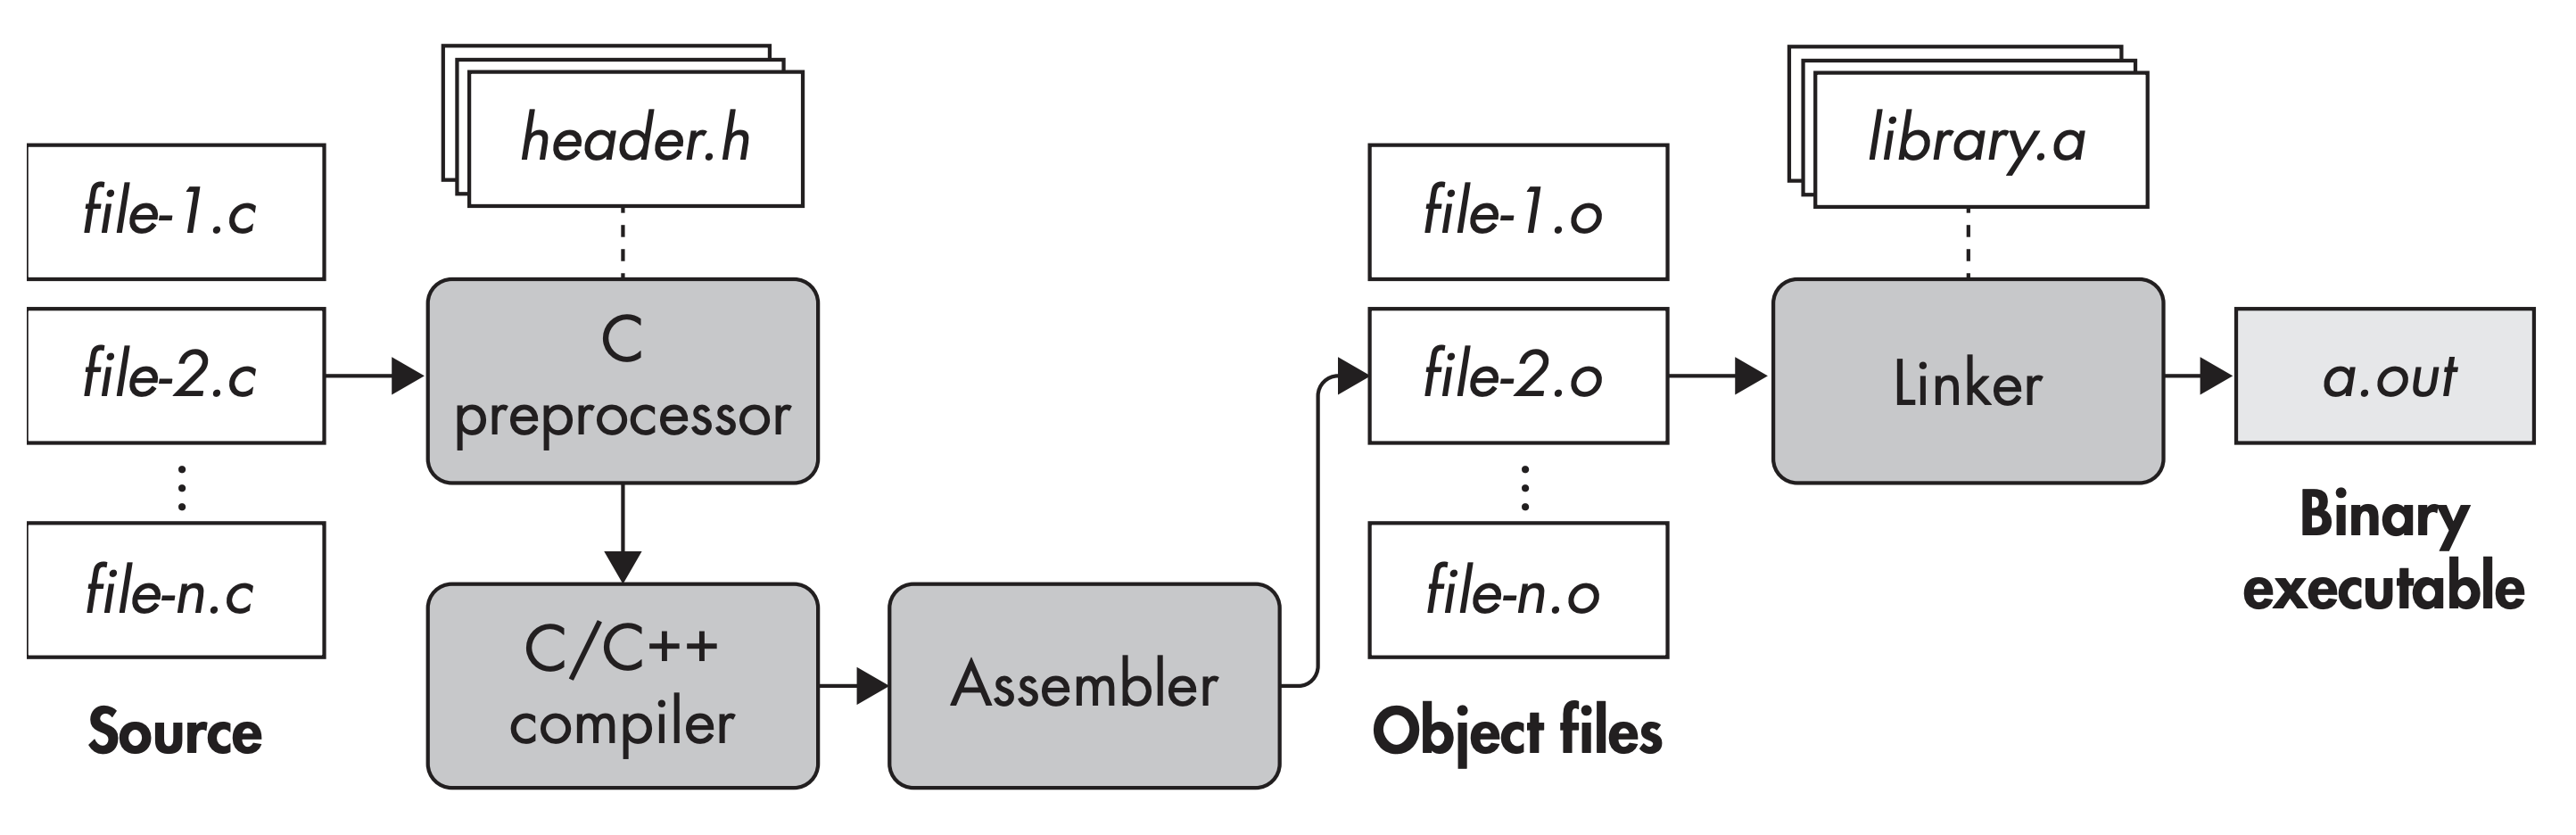
\includegraphics[width=0.8\linewidth]{Images/Compilation.png}
    \caption{The C compilation process.}
    \label{fig:Compilation}
\end{figure}

\subsubsection{The Preprocessing Phase}
The compilation process starts with a number of source files that you want to compile (shown as file-1.c through file-n.c in Figure \ref{fig:Compilation}). It’s possible to have just one source file, but large programs are typically composed of many files. Not only does this make the project easier to manage, but it speeds up compilation because if one file changes, you only have to recompile that file rather than all of the code. \\
C source files contain macros (denoted by \#define) and \#include directives. You use the \#include directives to include header files (with the extension .h) on which the source file depends. The preprocessing phase expands any \#define and \#include directives in the source file so all that’s left is pure C code ready to be compiled.

\subsubsection{The Compilation Phase}
After the preprocessing phase is complete, the source is ready to be compiled. The compilation phase takes the preprocessed code and translates it into assembly language. \\
The reason why the compilation phase produces assembly language and not machine code is because, due to the high number of popular compiled languages (like C, C++, Objective-C, Common Lisp, Delphi, Go, and Haskell), writing a compiler that directly emits machine code for each of these languages would be an extremely demanding and time-consuming task. It’s better to instead emit assembly code and have a single dedicated assembler that can handle the final translation of assembly to machine code for every language. \\
So, the output of the compilation phase is assembly, in reasonably human-readable form, with symbolic information intact.

\subsubsection{The Assembly Phase}
The input of the assembly phase is the set of assembly language files generated in the compilation phase, and the output is a set of object files, sometimes also referred to as modules. Object files contain machine instructions that are in principle executable by the processor.

\subsubsection{The Linking Phase}
The linking phase is the final phase of the compilation process. As the name implies, this phase links together all the object files into a single binary executable. \\
The program that performs the linking phase is called a linker, or link editor and it’s typically separate from the compiler, which usually implements all the preceding phases. \\
Object files are compiled independently from each other, preventing the compiler from assuming that an object will end up at any particular base address. Moreover, object files may reference functions or variables in other object files or in libraries that are external to the program. Before the linking phase, the addresses at which the referenced code and data will be placed are not yet known, so the object files only contain relocation symbols that specify how function and variable references should eventually be resolved. In the context of linking, references that rely on a relocation symbol are called symbolic references. When an object file references one of its own functions or variables by absolute address, the reference will also be symbolic. \\
The linker’s job is to take all the object files belonging to a program and merge them into a single coherent executable, typically intended to be loaded at a particular memory address.

\subsection{Symbols and Stripped Binaries}
High-level source code, such as C code, centers around functions and variables with meaningful, human-readable names. When compiling a program, compilers emit symbols, which keep track of such symbolic names and record which binary code and data correspond to each symbol. For instance, function symbols provide a mapping from symbolic, high-level function names to the first address and the size of each function. This information is normally used by the linker when combining object files and also aids debugging. \\
Unfortunately, extensive debugging information typically isn't included
in production-ready binaries, and even basic symbolic information is often
stripped to reduce file sizes and prevent reverse engineering, especially in
the case of malware or proprietary software.

\subsection{The ELF Format}
Executable and Linkable Format (ELF) is the default binary format on Linux-based systems and is used for executable files, object files, shared libraries, and core dumps. \\
Every ELF file starts with an executable header, which is just a structured series of bytes telling you that it’s an ELF file, what kind of ELF file it is, and where in the file to find all the other contents. \\
The code and data in an ELF binary are logically divided into contiguous non-overlapping chunks called sections. Sections don’t have any predetermined structure and are described by a section header, which denotes the properties of the section and allows you to locate the bytes belonging to the section. The section headers for all sections in the binary are contained in the section header table. \\
The program header table provides a segment view of the binary, as opposed to the section view provided by the section header table. The section view of an ELF binary is meant for static linking purposes only. In contrast, the segment view is used by the operating system and dynamic linker when loading an ELF into a process for execution to locate the relevant code and data and decide what to load into virtual memory.

\begin{figure}[H]
    \centering
    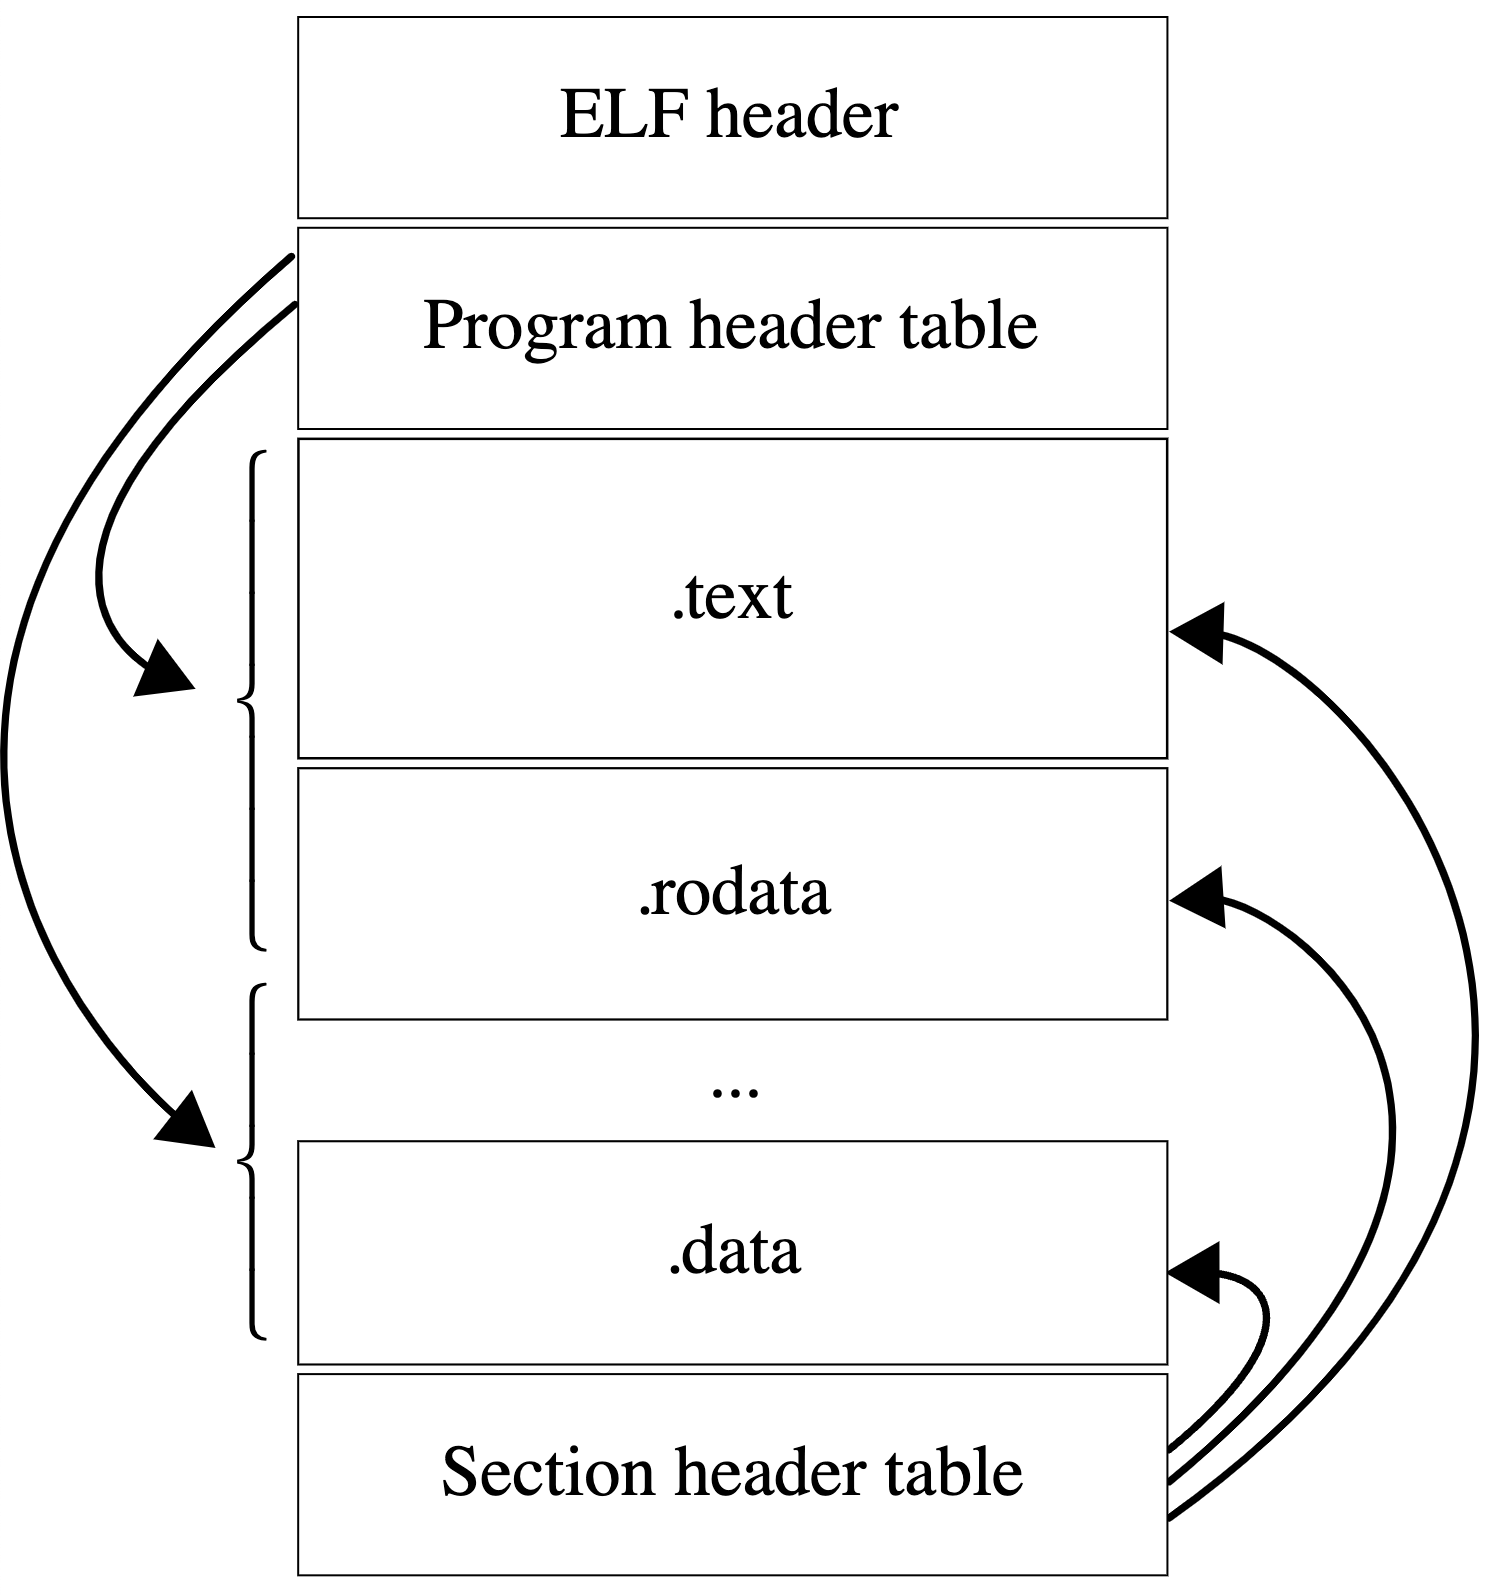
\includegraphics[width=0.45\linewidth]{Images/ELF.png}
    \caption{Structure of an ELF file.}
    \label{fig:ELF}
\end{figure}

\section{Static Analysis}
Static analysis describes the process of analyzing the code or structure of a program to determine its function. The program itself is not run at this time in contrast of when performing dynamic analysis.

\subsection{Antivirus Scanning}
When first analyzing prospective malware, a good first step is to run it through multiple antivirus programs, which may already have identified it. But antivirus tools are certainly not perfect. They rely mainly on a database of identifiable pieces of known suspicious code (file signatures), as well as behavioral and pattern-matching analysis (heuristics) to identify suspect files. One problem is that malware writers can easily modify their code, thereby changing their program’s signature and evading virus scanners. Also, rare malware often goes undetected by antivirus software because it’s simply not in the database. Finally, heuristics, while often successful in identifying unknown malicious code, can be bypassed by new and unique malware.

\subsection{Hashing}
Hashing is a common method used to uniquely identify malware. The malicious software is run through a hashing program that produces a unique hash that identifies that malware. The most commonly used hash functions are Message-Digest Algorithm 5 (MD5), Secure Hash Algorithm 1 (SHA-1) and Secure Hash Algorithm 256 (SHA-256) (Section \ref{ch:SHA}). Once you have a unique hash for a piece of malware, you can use it as a label and to see if the file has already been identified online.

\subsection{Linked Libraries and functions}
One of the most useful pieces of information that we can gather about an executable is the list of functions that it imports. Imports are functions used by one program that are actually stored in a different program, such as code libraries that contain functionality common to many programs. Code libraries can be connected to the main executable by linking. \\
Programmers link imports to their programs so that they don’t need to re-implement certain functionality in multiple programs. Code libraries can be linked statically, at runtime, or dynamically.

\begin{itemize}
    \item \textbf{Static Linking} - When a library is statically linked to an executable, all code from that library is copied into the executable, which makes the executable grow in size. When analyzing code, it’s difficult to differentiate between statically linked code and the executable’s own code.
    \item \textbf{Runtime Linking} - Executables that use runtime linking connect to libraries only when that function is needed, not at program start, as with dynamically linked programs. It is commonly used in malware, especially when it’s packed or obfuscated. 
    \item \textbf{Dynamic Linking} - When libraries are dynamically linked, the host OS searches for the necessary libraries when the program is loaded. When the program calls the linked library function, that function executes within the library.
\end{itemize}

\section{Disassembly}
When people say “disassembly” they usually mean static disassembly, which involves extracting the instructions from a binary without executing it. In contrast, dynamic disassembly, more commonly known as execution tracing, logs each executed instruction as the binary runs. The goal of every static disassembler is to translate all code in a binary into a form that a human can read or a machine can process (for further analysis). \\
There are two major approaches to static disassembly, each of which tries to avoid disassembly errors in its own way: linear disassembly and recursive disassembly. 

\subsection{Linear Disassembly}
Linear disassembly is conceptually the simplest approach. It iterates through all code segments in a binary, decoding all bytes consecutively and parsing them into a list of instructions. \\
The risk of using linear disassembly is that not all bytes may be instructions. For example, some compilers, such as Visual Studio, intersperse data such as jump tables with the code, without leaving any clues as to where exactly that data is. If disassemblers accidentally parse this inline data as code, they may encounter invalid opcodes, \textit{i.e.} the portion of a machine language instruction that specifies the operation to be performed.

\subsection{Recursive Disassembly}
Unlike linear disassembly, recursive disassembly is sensitive to control flow. It starts from known entry points into the binary and from there recursively follows control flow (such as jumps and calls) to discover code.  This allows recursive disassembly to work around data bytes in all but a handful of corner cases. The downside of this approach is that not all control flow is so easy to follow. For instance, it’s often difficult, if not impossible, to statically figure out the possible targets of indirect jumps or calls. \\
Recursive disassembly is the de facto standard in many reverse-engineering applications, such as malware analysis.

\subsection{Structuring Code}
There are various ways of structuring disassembled code that make the code easier to analyze in two ways:

\begin{itemize}
    \item \textbf{Compartmentalizing}: By breaking the code into logically connected chunks, it becomes easier to analyze what each chunk does and how chunks of code relate to each other.
    \item \textbf{Revealing control flow}: Some of the code structures I’ll discuss next explicitly represent not only the code itself but also the control transfers between blocks of code. These structures can be represented visually, making it much easier to quickly see how control flows through the code and to get a quick idea of what the code does.
\end{itemize}

\subsubsection{Functions}
In most high-level programming languages, functions are the fundamental building blocks used to group logically connected pieces of code. Programs that are well structured and properly divided into functions are much easier to understand than poorly structured programs. For this reason, most disassemblers make some effort to recover the original program’s function structure and use it to group disassembled instructions by function. This is known as function detection. \\
For binaries with symbolic information, function detection is trivial: the symbol table specifies the set of functions, along with their names, start addresses, and sizes. Unfortunately, many binaries are stripped of this information, which makes function detection far more challenging. \\
The predominant strategy that disassemblers use for function detection is based on function signatures, which are patterns of instructions often used at the start or end of a function. This strategy is used in all well-known recursive disassemblers.

\subsubsection{Control-Flow Graphs}
Breaking the disassembled code into functions is one thing, but some functions are quite large, which means analyzing even one function can be a complex task. To organize the internals of each function, disassemblers and binary analysis frameworks use another code structure, called a control-flow graph (CFG).

\begin{figure}[H]
    \centering
    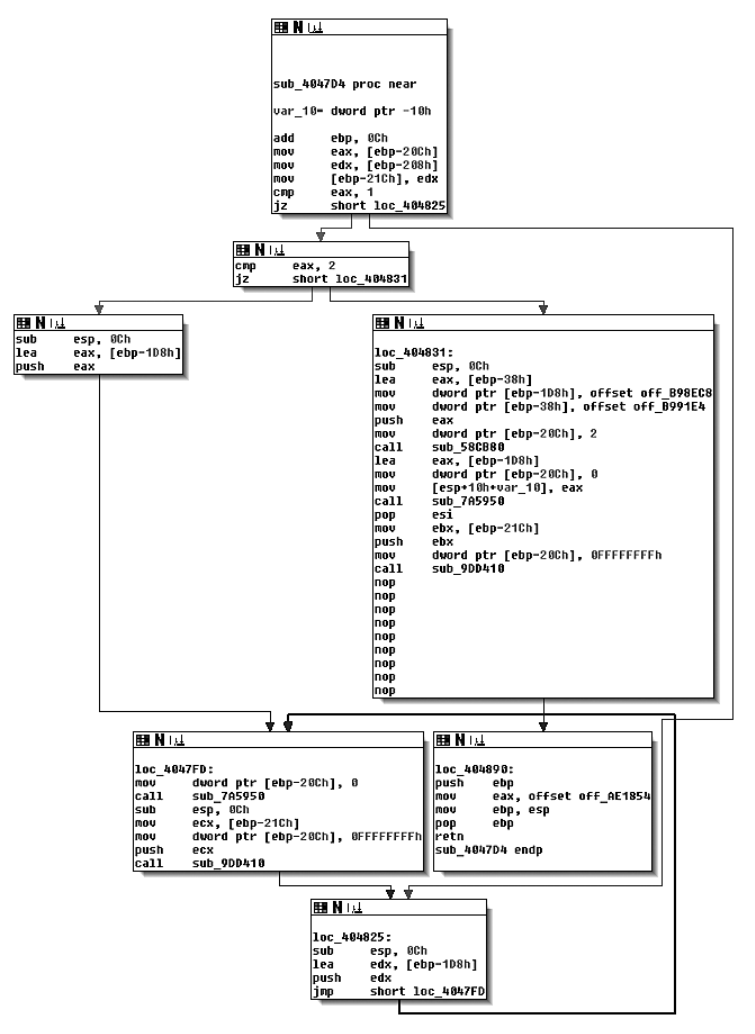
\includegraphics[width=0.6\linewidth]{Images/CFG.png}
    \caption{A CFG as seen in IDA Pro.}
    \label{fig:CFG}
\end{figure}

\noindent As you can see in Figure \ref{fig:CFG}, CFGs represent the code inside a function as a set of code blocks, called basic blocks, connected by branch edges, shown here as arrows. A basic block is a sequence of instructions, where the first instruction is the only entry point (the only instruction targeted by any jump in the binary), and the last instruction is the only exit point (the only instruction in the sequence that may jump to another basic block). \\
Call edges are not part of a CFG because they target code outside of the function. There is another code structure, called a call graph, that is designed to represent the edges between call instructions and functions.

\subsubsection{Call Graphs}
Call graphs are similar to CFGs, except they show the relationship between call sites and functions rather than basic blocks. In other words, CFGs show you how control may flow within a function, while call graphs show you which functions may call each other.

\begin{figure}[H]
    \centering
    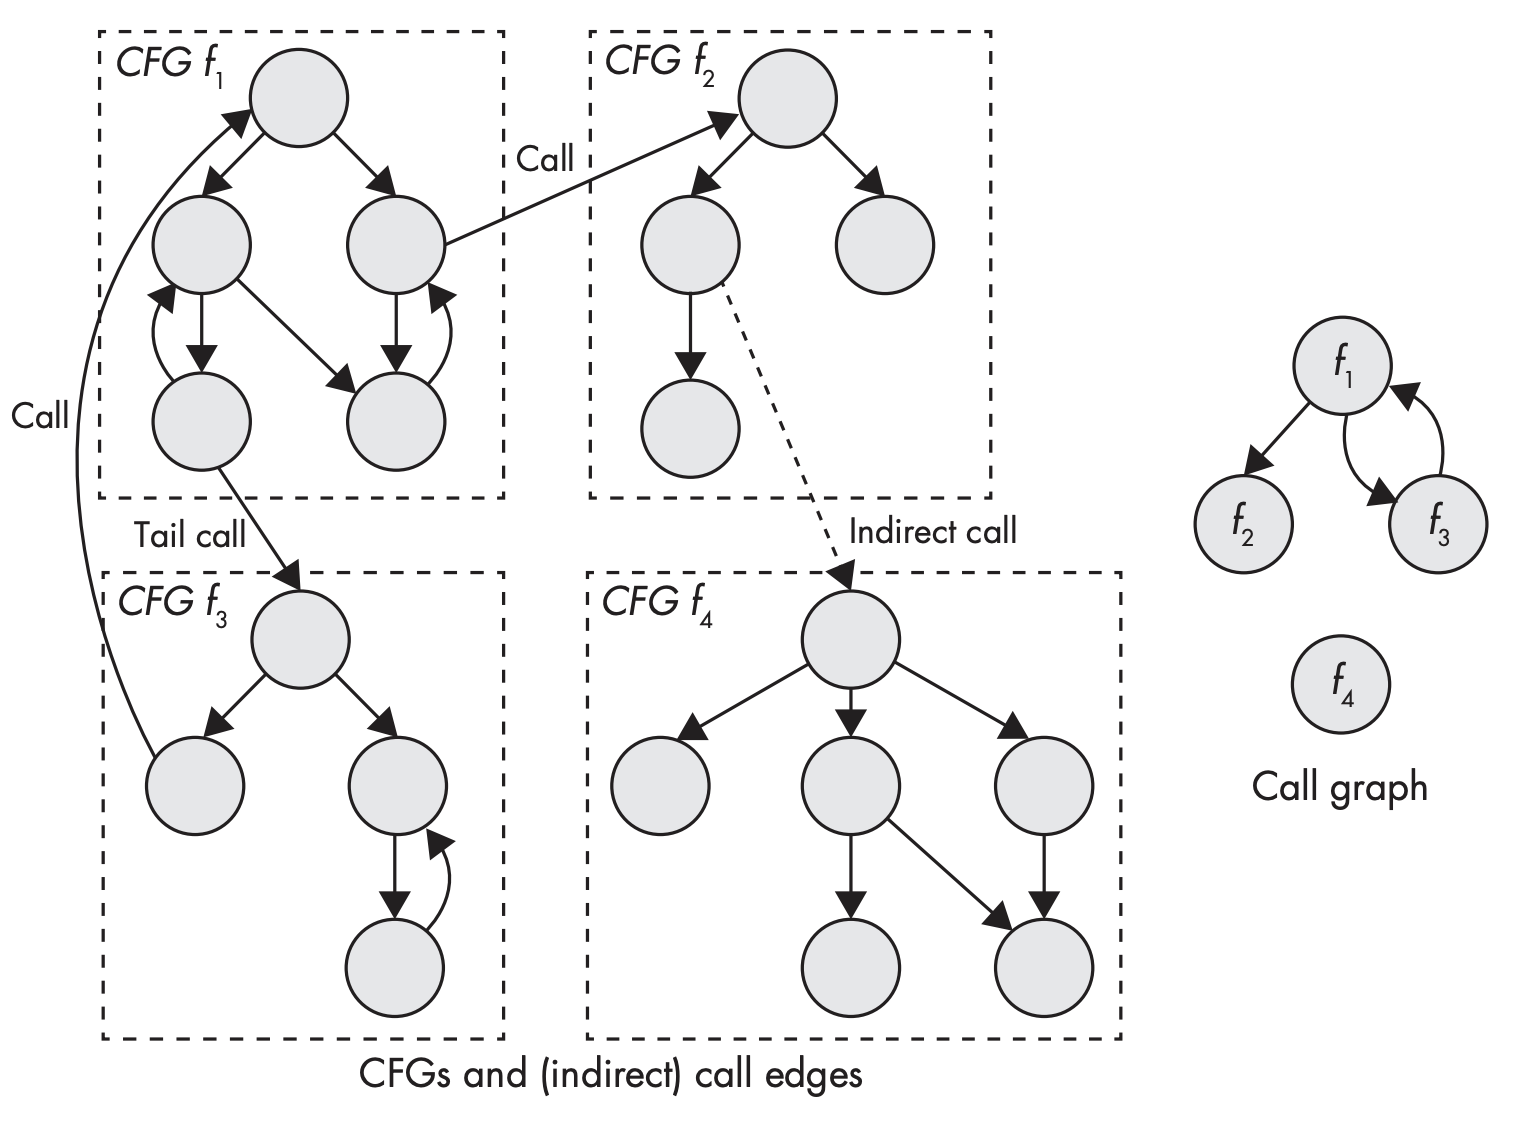
\includegraphics[width=0.8\linewidth]{Images/CallGraph.png}
    \caption{CFGs and connections between functions (left) and the corresponding call graph (right).}
    \label{fig:CallGraph}
\end{figure}

\section{Packed and Obfuscated Malware}
Malware writers often use packing or obfuscation to make their files more difficult to detect or analyze. Obfuscated programs are ones whose execution the malware author has attempted to hide. Packed programs are a subset of obfuscated programs in which the malicious program is compressed and cannot be analyzed. Both techniques will severely limit your attempts to statically analyze the malware.

\subsection{Obfuscation Techniques}
To explain the different existing obfuscation techniques we will use the article by Rabia Tahir "A Study on Malware and Malware Detection Techniques" \cite{tahir2018study} and the paper by You and Yim "Malware Obfuscation Techniques: A Brief Survey" \cite{you2010malware}. 

\subsubsection{Dead-Code Insertion}
This is easiest way to change code without affecting its meaning. In this technique, garbage code or statements are inserted in the code by using NOP statements and push followed by pop. These statements are used in such a sequence that it does not affect the semantics of code, while making the detection harder. 

\subsubsection{Instruction Replacement}
In this technique, instructions are replaced with other instructions that generate the same meaning just like synonyms in natural languages. For example all following instructions have the same effect on register eax: set the register value to zero.

\begin{lstlisting}
    move eax,0
    xor eax,eax
    and eax,0
    sub eax,eax
\end{lstlisting}

\noindent Since instruction are substituted with equivalent ones, this technique makes the detection of a malware very hard.

\subsubsection{Register Reassignment}
This technique reassign register in every copy without changing the semantics of the virus. It is a simple technique but when combine with other technique can make detection very difficult.

\subsubsection{Subroutine Reordering}
A set of instructions in a piece of code is permuted so that the code changes in its appearance while keeping the same behavior. An example of a subroutine followed by its reordering is shown below:

\begin{lstlisting}
    //Subroutine
    mov eax,0A
    push ecx
    add esi,ebx
    //Reordering
    add esi,ebx
    mov eax,0A
    push ecx
\end{lstlisting}

\subsubsection{Code Transposition}
Code transposition reorders the sequence of the instructions of an original code without having any impact on its behavior. There are two methods to achieve this technique. \\
The first method randomly shuffles the instructions, and then recovers the original execution order by inserting the unconditional branches or jumps. It is not difficult to defeat this method because the original program can be easily restored by removing the unconditional branches or jumps. On the other hand, the second method creates new generations by choosing and reordering the independent instructions that have no impact on one another. Because it is a complex problem to find the independent instructions, this method is hard to implement, but can make the cost of detection high. 

\subsubsection{Code Integration}
In code integration a malware knits itself to the code of its target program. In order to apply this technique, the target program is first decompiled into manageable objects, the malware is then seamlessly added between them, and then the integrated code is reassembled into a new generation. As one of the most sophisticated obfuscation techniques, code integration can make detection and recovery very difficult. 

\subsection{Packing Files}
When the packed program is run, a small wrapper program also runs to decompress the packed file and then run the unpacked file, as shown in Figure \ref{fig:Packed}. When a packed program is analyzed statically, only the small wrapper program can be dissected.

\begin{figure}[H]
    \centering
    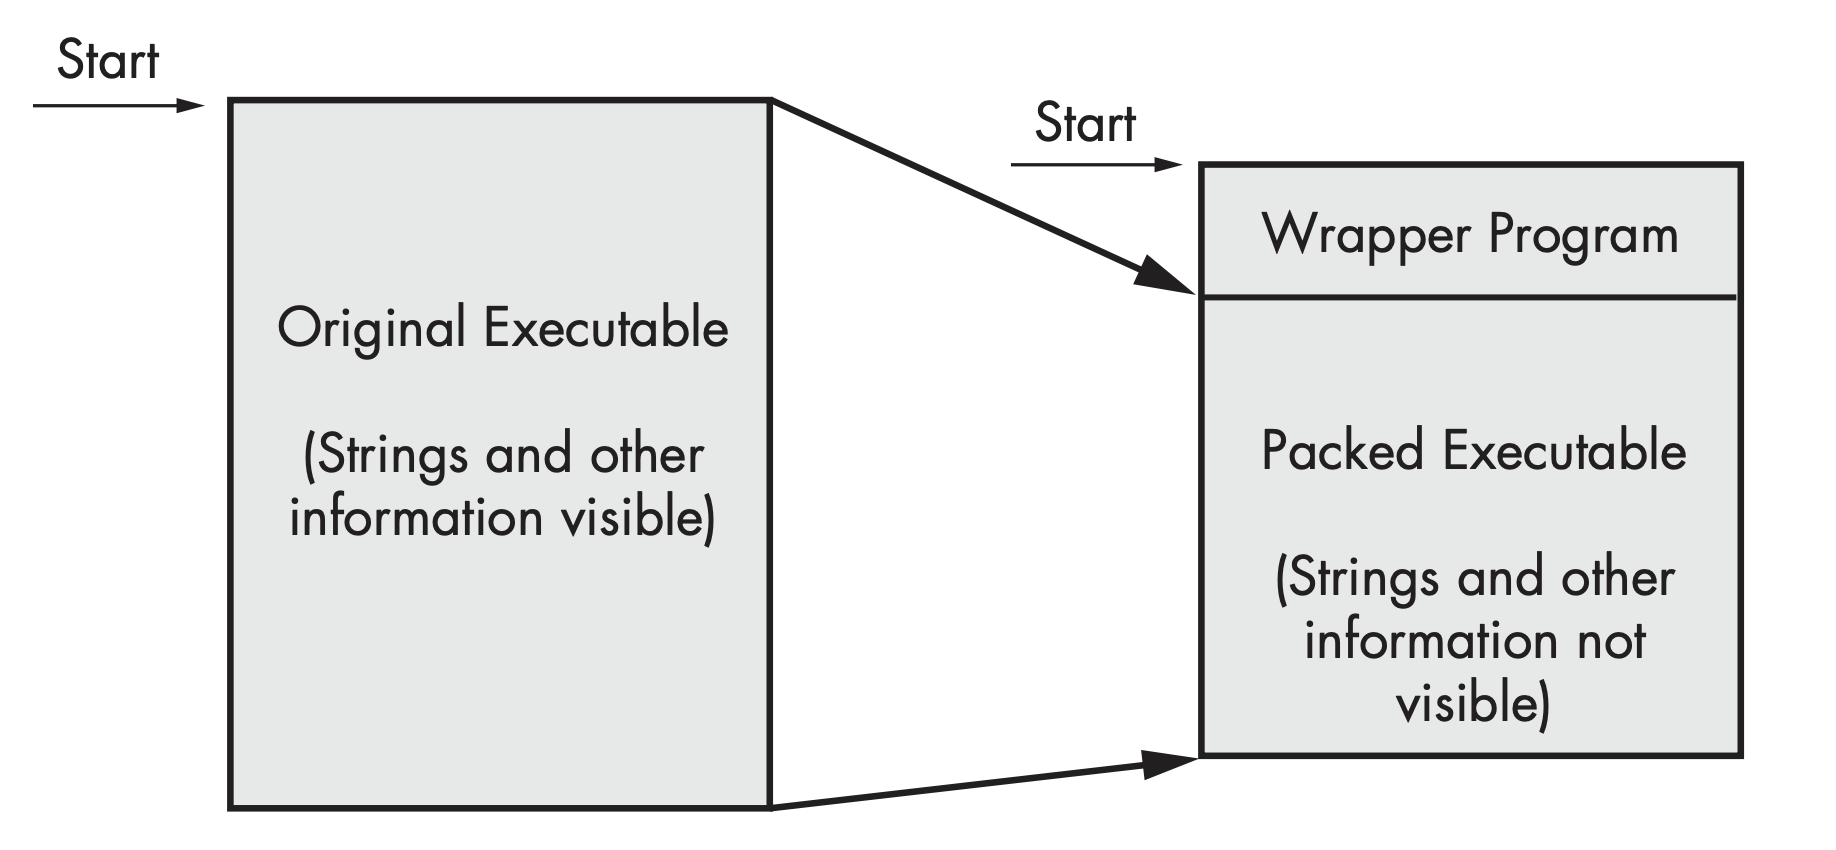
\includegraphics[width=0.7\linewidth]{Images/Packed.png}
    \caption{The file on the left is the original executable, with all strings, imports, and other information visible. On the right is a packed executable. All of the packed file’s strings, imports, and other information are compressed and invisible to most static analysis tools.}
    \label{fig:Packed}
\end{figure}